\documentclass{mylib/reporteCorto}

\title{Reporte}
\author{rodrigofranciscopablo }

\subject{Administración de proyectos de Software}
\mytitle{¿Cómo impacta la administración de proyectos de software en la calidad y ausencia de errrores en el software?}
\mysubTitle{Ensayo}
\students{Francisco Pablo \textsc{Rodrigo}}
\teacher{Ing. Gamboa Beltran \textsc{Jonahan}}
\group{1}
\deliverDate{6 de marzo de 2019}

\begin{document}

\coverPage

Los errores son un problema bastante común en el desarrollo de cualquier proyecto, por ejemplo, en la construcción de un edificio podrían fallar los cálculos de material necesario y por ende tendrían que parar la construcción. Otro ejemplo podría ser que en un proyecto de cableado estructurado alguna persona distraida podría pasar cable UTP de manera perpendicular a las líneas de transmisión eléctrica, lo cual provocaría ruido en la comunicación de los dispositivos finales que transmiten información a través del cable.\\

Los errores en el desarrollo de proyectos de software pueden provocar el mismo daño que un error en cualquier otro proyecto. Por ejemplo, si un sistema de control de frenos de un automóvil inteligente esta controlado por un ente de software. Si este sistema tiene un defecto y en lugar de frenar el automóvil cuando hay un objeto cerca acelera, indudablemente pude causar un efecto catasfrófico como mater a alguna persona.\\

Particularmente para el desarrollo de software existen tres tipos de errores:
\begin{itemize}
	\item De sintaxis
	\item De ejecución
	\item De lógica
\end{itemize}

Lo errores de sintaxis se refieren básicamente a que nuestro código fuente pase por un ente de software llamado compilador que verifica que no tengamos errores a la hora de escribir el programa. Los errores de ejecución se presentan una vez que se superó la fase de comiplación y se refieren al hecho de que un programa se cierre repentinamente realizando alguna tarea. Finalmente, los errores de lógica se refieren a que nuestro programa no muestre las salidas esperadas, por ejemplo si hacemos una calculadora e ingresamos $3 \times 4 $ y por alguna razón no obtenemos 12 sino otro valor.

\section*{¿Por qué se dan los errores?}

De acuerdo a lo explicado por el Ing. Julio del Razo en su conferencia de \textit{Ingeniería de Software} existen diversas razones de porque se da un error pero básicamente podríamos dividirlos en las siguientes.
\begin{itemize}
	\item Inconsistencia en la fase de toma de requerimentos.
	\item Incontabilidad.
	\item Errores de terceros.
	\item Omisión en la toma de requerimentos.
\end{itemize}	

Lo anterior indica que la \textbf{toma de requerimentos} es la parte más importante del desarrollo de software y por ello hay qu dedicarle gran parte de nuestro tiempo y no dar nada por hecho, es decir aclarar todos los puntos en los que podría haber discrepancia con el \textit{stakeholder}.

\section*{Regla 1-10-100}

Esta regla se refiere al costo de un proyecto de acuerdo a la fase en la que se encuentre. Por ejemplo si el proyecto se encuentra en las primeras fases (análisis o diseño) entonces reparar un error sería será relativamente sencillo por lo cual en la pirámide le corresponde el valor de 1. En cambio, si el proyecto ya esta en una fase intermedia como la \textit{implementación} entonces corregir un error podría costar más, y por último, si el proyecto ya esta concluido y en la fase de producción, reparar un error sería más complicado porque el sistema ya esta operando y tal vez ya perjudico a ciertos usuarios de la misma, el valor en la pirámide sería 100.

\begin{center}
	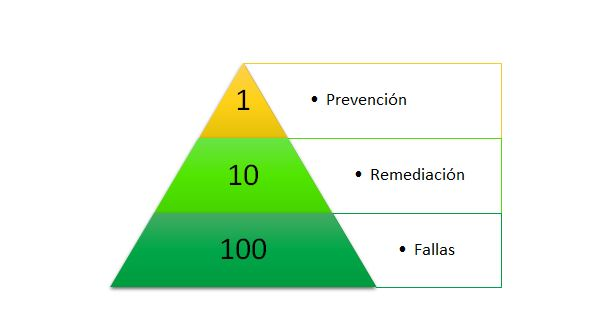
\includegraphics[scale=0.5]{img/admin/regla-1-10-100}
\end{center}

\section*{¿Que es la calidad de software?}

La calidad de software se define como la aptitud de un producto para ofrecer un alto grado de satisfacción a los clientes. También podríamos definirlo como la capacidad de nuestro ente de software a alinearse a los objetivos de la organización o del \textit{stakeholder}. Podemos observar que las definiciones anteriores no consideran aspectos técnicos, por ejemplo, si el proyecto se realizó con una \textit{programación espagethi} o cuestiones como escalabilidad, compatibilidad, etc.

\newpage

\section*{¿Cómo evitar errores?}

Finalmente, hablemos de \textit{\mytitle}.\\

La administración de proyectos de software nos permite construir una estructura de trabajo que será nuestra guía en la construcción de cualquier ente de software. Si tenemos un plan de los pasos a seguir para construir software de calidad entonces lo mejor será acatarlo para obtener los mejores resultados en nuestro proyecto. Dicho plan debe considerar como fases importantes la toma de requerimentos y la fase de pruebas ya que cualquier persona con conocimientos en computación podría desarrollar aplicaciones (ya sea web o móviles), pero no cualquier persona tendrá un proyecto estructurado y que considera fases de pruebas y de detección y correción de errores de una forma métodica. La \textit{\subject} nos permite tener la capacidad de considerar recursos (tiempos, costos, personal y herramientas) para poder hacer que los errores sean mínimos. 

Creo que lo que menos debemos hacer es convertirnos en desarrolladores de Windows y lanzar nuestra versión de \textit{producción} y esperar a que los usuarios reporten fallas para empezar a corregirlas ya que esto deja muy mala impresión de las personas que estan desarrollando la aplicación (de cualquier tipo; web, móvil, nativa).

El administrador del proyecto debe ser el encargado de monitorear el avance del proyecto ya sea con una metodología definida o de manera informal pero siempre debe de cuidar que el proyecto se este realizando con los recursos presupuestados y claro, definiendo una etapa o módulo de control de calidad. En la mayoría de los casos para los proyectos se opta por un monitoreo informal que permitirá hacerse una imagen clara del progreso del poryecto y con ello decidir si modificará sus recursos o los dejará de la manera que había planeado. Para el monitoreo se opta por la informalidad (\textit{metodologías ágiles}) porque es más rápido tanto para el desarrollador como para el administrador ya que el desarrollador no tiene que escribir largos y tediosos informes y el administrador no tiene que leerlos.

\section*{Conclusiones}

Los errores siempre serán un factor en cualquier proyecto de software dado que fueron hecho por humanos y los humanos tendemos de cometerlos en gran medida. Lo anterior no signifca que debamos tirar la tualla y dejar que un error forme parte del proyecto solo hace hincapié en un error se podría presentar en cualquier fase de desarrollo y es nuestro trabajo diseñar metodologías que nos permitan prevenir y corregir estos errores.

\end{document}
